\documentclass[11pt,aspectratio=43,svgnames]{beamer}

\usepackage{modules/cgs}

\begin{document} \maketitle

\begin{frame} \ft{Содержание}
	\tableofcontents
\end{frame}

\section{Теория некооперативных игр}

\begin{frame} \ft{Некооперативные игры}
Несколько участников одновременно принимают\\
решения и получают выигрыш в зависимости от\\
сочетания этих решений. Им известно, какой выигрыш\\
полагается за какие комбинации их действий. \medskip

Им доступен весь их опыт взаимодействия с миром\\
и друг с другом, но они не формируют коалиций\\
с жёстко зафиксированной стратегией.\\
Решение, как быть, они принимают\\
исключительно самостоятельно.
\end{frame}

\begin{frame} \ft{Актуальность теории}
Примеры таких взаимодействий встречаются\\
повсеместно: в экономике, в биологии, в дорожном\\
движении, в планировании мероприятий,\\
в криптовалюте\quad{\scriptsize\cite{caginalpCryptoNash}} \medskip

Задача теории~— предсказывать доли популяции,\\
выбирающие определённую стратегию.
\end{frame}

\section{Битва в море Бисмарка}

\begin{frame} \ft{Битва в море Бисмарка}
	Генерал Имамура может послать конвой\\
	северным маршрутом (2 дня) или\\
	южным маршрутом (3 дня).
	\medskip

	Генерал Кенни хочет бомбить конвой;\\
	если он отправит свои самолёты {\it не туда,}\\
	у него будет на это полдня меньше.\quad{\scriptsize\cite{petersGT}}
\end{frame}


\newcommand{\bismarckPO}{\gamePayoffs{2}{-2}{2.5}{-2.5}{1.5}{-1.5}{3}{-3}}


\begin{frame} \ft{Запись игры с помощью таблицы}
Кенни выбирает строку таблицы, Имамура выбирает\\
столбец. Их выигрыши записаны в соотв. клетках\\
таблицы напротив их выбора.
\begin{center} \begin{tikzpicture}[scale=0.44]
	\gameLines
	\gameNames{Кенни}{Имамура}
	\gameActions{Север}{Юг}
	\bismarckPO	
\end{tikzpicture} \end{center}
\end{frame}


\begin{frame} \ft{Доминирующая стратегия}
При любом действии Кенни Имамуре выгоднее\\
выбирать север (см. строчки).\\
У Имамуры есть домин.\:стратегия, у Кенни нет.
\begin{center} \begin{tikzpicture}[scale=0.44]
	\gameLines
	\gameNames{Кенни}{Имамура}
	\gameActions{Север}{Юг}
	\bismarckPO
	\obvod{-1.5}{3}{3.5}{3}{fill1}{0.5}{0}{\geqslant}
	\obvod{-1.5}{-1}{3.5}{-1}{fill1}{0.5}{0}{\geqslant}
\end{tikzpicture} \end{center}
\end{frame}


\begin{frame} \ft{Равновесие Нэша}
Умный Кенни тоже выберет север. Позиция\\
\(\lr*{\text{Север},\text{Север}}\)~— {\it равновесие Нэша}: действие \\
каждого~— лучший ответ на действие другого.
\begin{center} \begin{tikzpicture}[scale=0.44]
	\fill[p9480u,opacity=0.3] (0,0) rectangle (-5,4);
	\gameLines
	\gameNames{Кенни}{Имамура}
	\gameActions{Север}{Юг}
	\bismarckPO
	\obvod{-1.5}{3}{3.5}{3}{fill1}{0.5}{0}{\geqslant}
	\obvod{-3.5}{-3}{-3.5}{1}{fill3}{0.5}{-90}{\geqslant}
\end{tikzpicture} \end{center}
\end{frame}


\begin{frame} \ft{Равновесие Нэша}
	Равновесие Нэша~— это {\it устойчивое состояние\\
	общества,} такой закон, который никто\\
	не будет хотеть нарушить даже при\\
	отсутствии какого-либо контроля.
\end{frame}


\section{Кто такой Джон Нэш}

\begin{frame} \ft{Джон Форбс Нэш}

  \begin{center} \begin{tabular}{ll}
	\begin{minipage}{3.5cm}
		\includegraphics[width=3.2cm]{img/jn}
	\end{minipage}
   &
  	\begin{minipage}{7cm}
  		Первый в мире лауреат Абелевской \\
  		и Нобелевской премий (по экономике, \\
  		{\it «За анализ равновесия»).} \medskip

		Страдал шизофренией, которую \\
		сам научился подавлять.
  	\end{minipage}
  \end{tabular} \end{center}
\end{frame}

\section{Золотые шары (дилемма заключённого)}

\begin{frame} \ft{Что такое дилемма заключённого?}
	Известная игра, где равновесие Нэша\\
	находится не в позиции, которая\\
	кажется предпочтительной\\
	для обоих игроков.\quad{\scriptsize\cite{petersGT,mszGT}}
	\medskip

	Адаптирована в качестве телешоу\\
	«Золотые шары» на британском\\
	канале {\it ITV.}\quad{\scriptsize\cite{zurichGB}}
\end{frame}


\newcommand{\gbPO}{\gamePayoffs{5}{5}{0}{10}{10}{0}{0}{0}}


\begin{frame} \ft{Таблица выигрышей для «З.~Ш.»}
	Оба делятся~— выигрыш делится поровну.\\
	Один делится~— всё забирает другой.\\
	Оба хотят забрать~— остаются ни с чем.
\begin{center} \begin{tikzpicture}[scale=0.44]
	\gameLines
	\gameNames{Игрок 1}{Игрок 2}
	\gameActions{Делить}{Забрать}
	\gbPO
\end{tikzpicture} \end{center}
\end{frame}


\begin{frame} \ft{Что тут происходит?}
	У обоих игроков есть доминирующая\\
	стратегия: забирать деньги.\\
	Она всегда даёт не меньший выигрыш.
\begin{center} \begin{tikzpicture}[scale=0.44]
	\gameLines
	\gameNames{Игрок 1}{Игрок 2}
	\gameActions{Делить}{Забрать}
	\gbPO
	\obvod{-1.5}{3}{3.5}{3}{fill1}{0.5}{0}{\leqslant}
	\obvod{-1.5}{-1}{3.5}{-1}{fill1}{0.5}{0}{\leqslant}
\end{tikzpicture} \end{center}
\end{frame}


\begin{frame} \ft{Равновесие Нэша}
	В этой игре три равновесия Нэша,\\
	но ни одно из них~— не\\
	\(\lr*{\text{Делить},\text{Делить}}\).
\begin{center} \begin{tikzpicture}[scale=0.44]
	\fill[p9480u,opacity=0.3] (0,0) rectangle (5,-4)
		(0,0) rectangle (5,4) (0,0) rectangle (-5,-4);
	\gameLines
	\gameNames{Игрок 1}{Игрок 2}
	\gameActions{Делить}{Забрать}
	\gbPO
	\obvod{-1.5}{-1}{3.5}{-1}{fill1}{0.44}{0}{=}
	\obvod{-1.5}{3}{3.5}{3}{fill1}{0.44}{0}{\leqslant}
	\obvod{1.5}{-3}{1.5}{1}{fill3}{0.44}{-90}{=}
	\obvod{-3.5}{-3}{-3.5}{1}{fill3}{0.44}{-90}{\leqslant}
\end{tikzpicture} \end{center}
\end{frame}


\begin{frame} \ft{Парето-оптимум}
	Участники пытаются разработать такую\\
	систему контроля, которая бы заставила их\\
	гарантированно находиться в позиции,\\
	оптимальной по Парето:
	\medskip
	
	Нельзя улучшить чей-либо выигрыш,\\
	не ухудшив суммарного выигрыша и\\
	справедливости его распределения.
\end{frame}


\section{Уступить или проехать (Ястребы и голуби)}

\newcommand{\yieldPO}{\gamePayoffs{-1}{-1}{1}{2}{2}{1}{-11}{-11}}


\begin{frame} \ft{Уступить или проехать: выигрыши}
	Оба уступают~— заминка на одном месте\\
	Один уступает~— оба счастливы\\
	Оба едут~— попадают в ДТП
\begin{center} \begin{tikzpicture}[scale=0.44]
	\gameLines
	\gameNames{Игрок 1}{Игрок 2}
	\gameActions{Уступить}{Ехать}
	\yieldPO
\end{tikzpicture} \end{center}
\end{frame}


\begin{frame} \ft{Доминирующая стратегия}
	Ни у одного из игроков нет\\
	доминирующей стратегии. (Игра симметрична,\\
	поэтому покажем только для первого.)
\begin{center} \begin{tikzpicture}[scale=0.44]
	\gameLines
	\gameNames{Игрок 1}{Игрок 2}
	\gameActions{Уступить}{Ехать}
	\yieldPO
	\obvod{-1.5}{3}{3.5}{3}{fill1}{0.5}{0}{\leqslant}
	\obvod{-1.5}{-1}{3.5}{-1}{fill1}{0.5}{0}{\geqslant}
\end{tikzpicture} \end{center}
\end{frame}


\begin{frame} \ft{Два равновесия Нэша и светофор}
	Есть два симметричных равновесия Нэша,\\
	от которых игрокам невыгодно отступать,\\
	если им указать, в какой они играют.
\begin{center} \begin{tikzpicture}[scale=0.44]
	\fill[p9480u,opacity=0.3] (0,0) rectangle (5,4)
		(0,0) rectangle (-5,-4);
	\gameLines
	\gameNames{Игрок 1}{Игрок 2}
	\gameActions{Уступить}{Ехать}
	\yieldPO
	\obvod{-1.5}{3}{3.5}{3}{fill1}{0.5}{0}{\leqslant}
	\obvod{1.5}{-3}{1.5}{1}{fill3}{0.5}{90}{\leqslant}
\end{tikzpicture} \end{center}
\end{frame}


\begin{frame} \ft{Два равновесия Нэша и светофор}
	Прибор, который это указывает, \\
	называется {\it светофор.} Но предлагается\\
	поискать равновесие ещё кое-где.
\begin{center} \begin{tikzpicture}[scale=0.44]
	\fill[p9480u,opacity=0.3] (0,0) rectangle (5,4)
		(0,0) rectangle (-5,-4);
	\gameLines
	\gameNames{Игрок 1}{Игрок 2}
	\gameActions{Уступить}{Ехать}
	\yieldPO
	\obvod{-1.5}{-1}{3.5}{-1}{fill1}{0.5}{0}{\geqslant}
	\obvod{-3.5}{-3}{-3.5}{1}{fill3}{0.5}{-90}{\leqslant}
\end{tikzpicture} \end{center}
\end{frame}


\section{Смешанные стратегии}

\begin{frame} \ft{Суть смешанных стратегий}
	Пусть {\it абстрактный коллективный} первый игрок\\
	уступает с вероятностью \(p\), а второй~— с вероятностью \(q\).\medskip

	Равновесие Нэша~— позиция, когда действие каждого\\
	игрока~— {\it лучший ответ} на действие другого.\medskip

	Найдём, какая \(q\) будет лучшим ответом\\
	в зависимости от \(p\).
\end{frame}


\begin{frame} \ft{Ожидаемый выигрыш второго игрока}
   \vphantom{t}\centerline{
	\(-1\cdot pq +2\cdot p\lr*{1-q} +1\cdot \lr*{1-p}q -11\cdot \lr*{1-p}\lr*{1-q} =\)} \\
   \vphantom{t}\centerline{
	\(= \lr*{12 - 15 p} \cdot q + 13 p - 11\)}\\
	Лучшая \(q\)~— либо 0, либо 1, либо {\it все возможные.}
\begin{center} \begin{tikzpicture}[scale=0.44]
	\gameLines
	\gameNames{Игрок 1}{Игрок 2}
	\gameActions{Уступить}{Ехать}
	\yieldPO
\end{tikzpicture} \end{center}
\end{frame}


\begin{frame} \ft{{\it Три} равновесия Нэша}
	\( p < \frac45 \), тогда \(q=1\)\\
	\( p = \frac45 \), тогда \(q\) любое, выигрыш от него не зависит\\
	\( p < \frac45 \), тогда \(q=0\)
\begin{center} \begin{tikzpicture}[scale=3.35]
\draw[thick,->] (-0.2,0) -- (1.2,0) node[below]{\(p\)};
\draw[thick,->] (0,-0.2) -- (0,1.2) node[left]{\(q\)};

\foreach \t / \ttext in {1, 0.5 / \frac12, 0.8 / \frac45} {
  \draw (\t,0.05) -- (\t,-0.05) node[below,fill=dgray,
        inner sep=0.3ex,text height=2.2ex]{$\ttext$};
  \draw (0.05,\t) -- (-0.05,\t) node[left, fill=dgray,
        inner sep=0.3ex,text height=2.2ex]{$\ttext$};}
  \draw (0,-0.05) node[below,fill=dgray,
        inner sep=0.3ex,text height=2.2ex]{$0$};

\draw[very thick,fill1,line cap=round] (0,1) -- (0.8,1) -- (0.8,0) -- (1,0);
\draw[very thick,fill3,line cap=round] (1,0) -- (1,0.8) -- (0,0.8) -- (0,1);

\foreach \x / \y in {0 / 1, 0.8 / 0.8, 1 / 0} {
   \fill[PaleVioletRed,fill opacity=0.85] (\x , \y) circle[radius=0.4mm];}
\end{tikzpicture} \end{center}
\end{frame}


\section{Эволюционная теория игр}

\begin{frame} \ft{Модель репликации}
Большая популяция людей каждый день играет \\
в «уступить или проехать» внутри себя. Каждый \\
человек либо целый день всех пропускает, \\
либо целый день едет первым.

Каждый вечер каждый человек \(i\) выбирает своего \\
случайного соседа \(j\), и если тот в течение дня получил \\
б\'oльший выигрыш, чем \(i\), то \(i\) на следующий день \\
с некоторой вероятностью начинает играть так, \\
как \(j\) играл сегодня.\quad{\scriptsize\cite{brusselsEVO}}
\end{frame}


\begin{frame} \ft{Вероятность смены стратегии}
Эта вероятность равна
	\[\frac{P(j) - P(i)}{\lr*{11+2} \cdot \max\lr*{d(j),d(i)}}\]

{\it Смешанную стратегию} мы мыслим как долю людей, \\
которые сегодня всем уступают.

Чем больший выигрыш получают люди, играющие \\
определённым образом, тем быстрее растёт \\
их количество.\quad{\scriptsize\cite{derivativeEVO}}
\end{frame}


\begin{frame} \ft{Доля людей, которые уступают дорогу}
	Доля людей, которые уступают дорогу, стремится \\
	к \(p = \frac45\) из равновесия Нэша.

	\documentclass[a4paper,11pt]{article}

\usepackage[margin=1cm]{geometry}

\parskip = 5mm

\usepackage{tikz}

\begin{document}

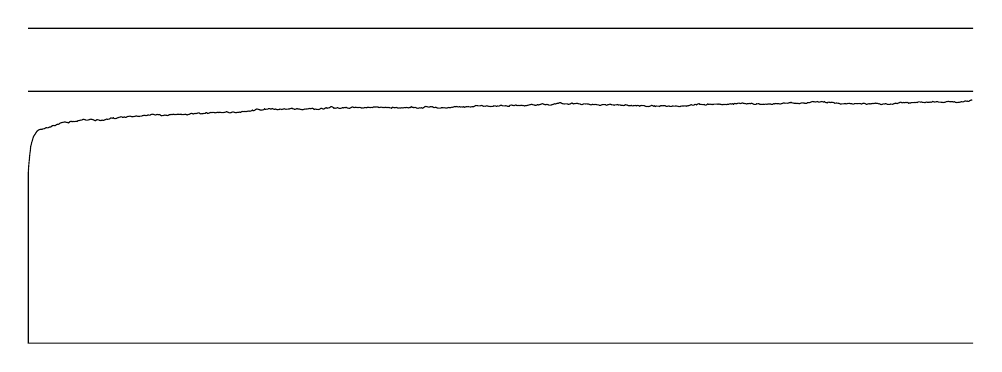
\begin{tikzpicture}
\draw (0,4) -- (12,4) (12,4 * 0.800000) -- (0,4 * 0.800000) (12,0) -- (0,0)-- (0.000000, 2.163846) -- (0.010909, 2.304231) -- (0.021818, 2.410000) -- (0.032727, 2.502692) -- (0.043636, 2.546538) -- (0.054545, 2.582692) -- (0.065455, 2.621154) -- (0.076364, 2.638462) -- (0.087273, 2.653846) -- (0.098182, 2.671923) -- (0.109091, 2.689231) -- (0.120000, 2.699615) -- (0.130909, 2.707692) -- (0.141818, 2.711923) -- (0.152727, 2.716154) -- (0.163636, 2.717692) -- (0.174545, 2.716154) -- (0.185455, 2.721923) -- (0.196364, 2.721538) -- (0.207273, 2.724615) -- (0.218182, 2.733077) -- (0.229091, 2.737308) -- (0.240000, 2.734615) -- (0.250909, 2.735000) -- (0.261818, 2.740769) -- (0.272727, 2.746923) -- (0.283636, 2.745769) -- (0.294545, 2.750769) -- (0.305455, 2.761538) -- (0.316364, 2.763077) -- (0.327273, 2.765769) -- (0.338182, 2.760769) -- (0.349091, 2.768077) -- (0.360000, 2.775769) -- (0.370909, 2.780769) -- (0.381818, 2.779615) -- (0.392727, 2.783846) -- (0.403636, 2.794231) -- (0.414545, 2.798077) -- (0.425455, 2.801154) -- (0.436364, 2.804231) -- (0.447273, 2.806923) -- (0.458182, 2.808462) -- (0.469091, 2.810385) -- (0.480000, 2.806154) -- (0.490909, 2.804231) -- (0.501818, 2.801923) -- (0.512727, 2.797692) -- (0.523636, 2.808846) -- (0.534545, 2.815769) -- (0.545455, 2.818846) -- (0.556364, 2.811923) -- (0.567273, 2.816538) -- (0.578182, 2.814615) -- (0.589091, 2.814615) -- (0.600000, 2.816923) -- (0.610909, 2.818462) -- (0.621818, 2.815769) -- (0.632727, 2.825385) -- (0.643636, 2.826538) -- (0.654545, 2.829231) -- (0.665455, 2.833846) -- (0.676364, 2.832308) -- (0.687273, 2.836538) -- (0.698182, 2.844615) -- (0.709091, 2.841538) -- (0.720000, 2.839231) -- (0.730909, 2.833462) -- (0.741818, 2.832308) -- (0.752727, 2.832308) -- (0.763636, 2.835385) -- (0.774545, 2.837692) -- (0.785455, 2.843846) -- (0.796364, 2.845000) -- (0.807273, 2.843462) -- (0.818182, 2.840000) -- (0.829091, 2.835000) -- (0.840000, 2.831923) -- (0.850909, 2.824615) -- (0.861818, 2.831923) -- (0.872727, 2.837692) -- (0.883636, 2.836538) -- (0.894545, 2.835385) -- (0.905455, 2.829615) -- (0.916364, 2.828077) -- (0.927273, 2.828077) -- (0.938182, 2.833846) -- (0.949091, 2.830000) -- (0.960000, 2.831154) -- (0.970909, 2.835385) -- (0.981818, 2.838846) -- (0.992727, 2.846538) -- (1.003636, 2.844615) -- (1.014545, 2.844615) -- (1.025455, 2.845000) -- (1.036364, 2.850000) -- (1.047273, 2.860000) -- (1.058182, 2.859231) -- (1.069091, 2.857308) -- (1.080000, 2.863462) -- (1.090909, 2.853462) -- (1.101818, 2.851538) -- (1.112727, 2.853077) -- (1.123636, 2.856538) -- (1.134545, 2.862308) -- (1.145455, 2.865000) -- (1.156364, 2.870385) -- (1.167273, 2.871923) -- (1.178182, 2.875385) -- (1.189091, 2.873846) -- (1.200000, 2.867308) -- (1.210909, 2.870385) -- (1.221818, 2.873846) -- (1.232727, 2.867692) -- (1.243636, 2.868846) -- (1.254545, 2.874615) -- (1.265455, 2.880769) -- (1.276364, 2.880000) -- (1.287273, 2.884231) -- (1.298182, 2.883077) -- (1.309091, 2.880000) -- (1.320000, 2.874231) -- (1.330909, 2.876538) -- (1.341818, 2.878846) -- (1.352727, 2.880769) -- (1.363636, 2.884615) -- (1.374545, 2.886538) -- (1.385455, 2.882308) -- (1.396364, 2.883462) -- (1.407273, 2.878846) -- (1.418182, 2.883846) -- (1.429091, 2.883846) -- (1.440000, 2.883846) -- (1.450909, 2.888462) -- (1.461818, 2.891923) -- (1.472727, 2.895000) -- (1.483636, 2.892692) -- (1.494545, 2.890769) -- (1.505455, 2.891154) -- (1.516364, 2.897308) -- (1.527273, 2.898077) -- (1.538182, 2.895385) -- (1.549091, 2.897308) -- (1.560000, 2.904231) -- (1.570909, 2.907308) -- (1.581818, 2.908846) -- (1.592727, 2.905769) -- (1.603636, 2.900385) -- (1.614545, 2.898077) -- (1.625455, 2.899615) -- (1.636364, 2.905769) -- (1.647273, 2.903462) -- (1.658182, 2.900769) -- (1.669091, 2.903846) -- (1.680000, 2.896154) -- (1.690909, 2.888077) -- (1.701818, 2.890385) -- (1.712727, 2.890385) -- (1.723636, 2.894231) -- (1.734545, 2.897692) -- (1.745455, 2.895385) -- (1.756364, 2.895385) -- (1.767273, 2.891923) -- (1.778182, 2.892692) -- (1.789091, 2.901154) -- (1.800000, 2.900769) -- (1.810909, 2.906154) -- (1.821818, 2.903462) -- (1.832727, 2.904231) -- (1.843636, 2.908462) -- (1.854545, 2.903846) -- (1.865455, 2.905385) -- (1.876364, 2.902308) -- (1.887273, 2.906154) -- (1.898182, 2.908077) -- (1.909091, 2.908077) -- (1.920000, 2.906154) -- (1.930909, 2.907308) -- (1.941818, 2.908846) -- (1.952727, 2.901923) -- (1.963636, 2.903077) -- (1.974545, 2.903846) -- (1.985455, 2.905385) -- (1.996364, 2.908462) -- (2.007273, 2.903462) -- (2.018182, 2.898077) -- (2.029091, 2.903846) -- (2.040000, 2.905385) -- (2.050909, 2.908846) -- (2.061818, 2.915000) -- (2.072727, 2.919615) -- (2.083636, 2.916154) -- (2.094545, 2.910000) -- (2.105455, 2.914615) -- (2.116364, 2.917308) -- (2.127273, 2.916923) -- (2.138182, 2.917692) -- (2.149091, 2.921923) -- (2.160000, 2.923846) -- (2.170909, 2.925000) -- (2.181818, 2.914615) -- (2.192727, 2.911538) -- (2.203636, 2.914231) -- (2.214545, 2.912308) -- (2.225455, 2.918077) -- (2.236364, 2.919231) -- (2.247273, 2.918462) -- (2.258182, 2.926923) -- (2.269091, 2.926154) -- (2.280000, 2.917308) -- (2.290909, 2.921154) -- (2.301818, 2.923462) -- (2.312727, 2.929615) -- (2.323636, 2.928846) -- (2.334545, 2.929231) -- (2.345455, 2.930769) -- (2.356364, 2.931923) -- (2.367273, 2.926923) -- (2.378182, 2.925000) -- (2.389091, 2.928846) -- (2.400000, 2.931538) -- (2.410909, 2.933846) -- (2.421818, 2.928077) -- (2.432727, 2.933846) -- (2.443636, 2.931538) -- (2.454545, 2.928077) -- (2.465455, 2.928462) -- (2.476364, 2.928462) -- (2.487273, 2.930769) -- (2.498182, 2.932692) -- (2.509091, 2.936154) -- (2.520000, 2.940385) -- (2.530909, 2.935769) -- (2.541818, 2.932308) -- (2.552727, 2.925000) -- (2.563636, 2.925000) -- (2.574545, 2.926923) -- (2.585455, 2.933846) -- (2.596364, 2.936154) -- (2.607273, 2.935385) -- (2.618182, 2.933462) -- (2.629091, 2.928077) -- (2.640000, 2.926538) -- (2.650909, 2.931538) -- (2.661818, 2.932308) -- (2.672727, 2.931923) -- (2.683636, 2.935769) -- (2.694545, 2.930769) -- (2.705455, 2.936154) -- (2.716364, 2.943462) -- (2.727273, 2.942308) -- (2.738182, 2.940769) -- (2.749091, 2.943462) -- (2.760000, 2.941538) -- (2.770909, 2.941154) -- (2.781818, 2.946923) -- (2.792727, 2.946154) -- (2.803636, 2.948846) -- (2.814545, 2.945769) -- (2.825455, 2.948077) -- (2.836364, 2.952308) -- (2.847273, 2.960769) -- (2.858182, 2.951154) -- (2.869091, 2.955385) -- (2.880000, 2.960769) -- (2.890909, 2.969231) -- (2.901818, 2.975769) -- (2.912727, 2.972692) -- (2.923636, 2.970000) -- (2.934545, 2.966538) -- (2.945455, 2.959231) -- (2.956364, 2.963077) -- (2.967273, 2.959231) -- (2.978182, 2.962692) -- (2.989091, 2.964231) -- (3.000000, 2.976154) -- (3.010909, 2.969615) -- (3.021818, 2.972692) -- (3.032727, 2.971538) -- (3.043636, 2.973462) -- (3.054545, 2.979231) -- (3.065455, 2.978846) -- (3.076364, 2.974231) -- (3.087273, 2.973077) -- (3.098182, 2.980000) -- (3.109091, 2.975385) -- (3.120000, 2.971923) -- (3.130909, 2.970000) -- (3.141818, 2.973846) -- (3.152727, 2.968846) -- (3.163636, 2.965000) -- (3.174545, 2.966154) -- (3.185455, 2.967692) -- (3.196364, 2.973846) -- (3.207273, 2.972692) -- (3.218182, 2.966923) -- (3.229091, 2.971538) -- (3.240000, 2.972692) -- (3.250909, 2.977308) -- (3.261818, 2.973077) -- (3.272727, 2.970769) -- (3.283636, 2.972308) -- (3.294545, 2.972308) -- (3.305455, 2.974615) -- (3.316364, 2.973462) -- (3.327273, 2.979231) -- (3.338182, 2.980385) -- (3.349091, 2.986154) -- (3.360000, 2.976923) -- (3.370909, 2.975385) -- (3.381818, 2.970385) -- (3.392727, 2.971923) -- (3.403636, 2.974231) -- (3.414545, 2.979615) -- (3.425455, 2.974231) -- (3.436364, 2.974615) -- (3.447273, 2.973462) -- (3.458182, 2.969231) -- (3.469091, 2.967308) -- (3.480000, 2.963846) -- (3.490909, 2.965769) -- (3.501818, 2.970000) -- (3.512727, 2.974615) -- (3.523636, 2.972692) -- (3.534545, 2.973846) -- (3.545455, 2.975000) -- (3.556364, 2.976154) -- (3.567273, 2.980000) -- (3.578182, 2.981154) -- (3.589091, 2.976154) -- (3.600000, 2.982692) -- (3.610909, 2.983462) -- (3.621818, 2.977308) -- (3.632727, 2.968077) -- (3.643636, 2.973846) -- (3.654545, 2.971538) -- (3.665455, 2.969231) -- (3.676364, 2.969615) -- (3.687273, 2.968077) -- (3.698182, 2.970385) -- (3.709091, 2.977308) -- (3.720000, 2.984231) -- (3.730909, 2.981154) -- (3.741818, 2.974615) -- (3.752727, 2.972692) -- (3.763636, 2.979231) -- (3.774545, 2.988462) -- (3.785455, 2.990385) -- (3.796364, 2.983462) -- (3.807273, 2.988846) -- (3.818182, 2.987308) -- (3.829091, 2.991923) -- (3.840000, 3.001923) -- (3.850909, 3.004231) -- (3.861818, 3.001154) -- (3.872727, 2.993846) -- (3.883636, 2.983462) -- (3.894545, 2.986538) -- (3.905455, 2.984231) -- (3.916364, 2.986923) -- (3.927273, 2.990385) -- (3.938182, 2.986923) -- (3.949091, 2.983846) -- (3.960000, 2.980769) -- (3.970909, 2.984231) -- (3.981818, 2.986538) -- (3.992727, 2.991538) -- (4.003636, 2.987308) -- (4.014545, 2.992692) -- (4.025455, 2.990385) -- (4.036364, 2.996538) -- (4.047273, 2.989231) -- (4.058182, 2.985385) -- (4.069091, 2.984231) -- (4.080000, 2.983462) -- (4.090909, 2.986538) -- (4.101818, 2.993462) -- (4.112727, 2.999615) -- (4.123636, 3.000000) -- (4.134545, 2.993846) -- (4.145455, 2.991923) -- (4.156364, 2.997308) -- (4.167273, 2.994615) -- (4.178182, 2.993077) -- (4.189091, 2.991154) -- (4.200000, 2.994231) -- (4.210909, 2.995385) -- (4.221818, 2.991154) -- (4.232727, 2.986154) -- (4.243636, 2.988077) -- (4.254545, 2.986154) -- (4.265455, 2.988846) -- (4.276364, 2.993077) -- (4.287273, 2.990769) -- (4.298182, 2.988846) -- (4.309091, 2.996538) -- (4.320000, 2.995769) -- (4.330909, 2.995385) -- (4.341818, 2.991154) -- (4.352727, 2.995000) -- (4.363636, 2.994231) -- (4.374545, 2.992308) -- (4.385455, 3.001154) -- (4.396364, 2.999615) -- (4.407273, 2.998846) -- (4.418182, 3.001154) -- (4.429091, 2.998462) -- (4.440000, 3.001154) -- (4.450909, 2.993846) -- (4.461818, 2.993846) -- (4.472727, 2.996538) -- (4.483636, 2.998462) -- (4.494545, 2.995385) -- (4.505455, 2.992308) -- (4.516364, 2.993077) -- (4.527273, 2.992692) -- (4.538182, 2.996154) -- (4.549091, 2.992308) -- (4.560000, 2.994615) -- (4.570909, 2.992308) -- (4.581818, 2.994231) -- (4.592727, 2.988077) -- (4.603636, 2.988846) -- (4.614545, 2.983077) -- (4.625455, 2.996538) -- (4.636364, 2.995000) -- (4.647273, 2.990000) -- (4.658182, 2.989615) -- (4.669091, 2.992308) -- (4.680000, 2.995000) -- (4.690909, 2.986154) -- (4.701818, 2.985769) -- (4.712727, 2.988846) -- (4.723636, 2.985769) -- (4.734545, 2.987308) -- (4.745455, 2.990385) -- (4.756364, 2.986923) -- (4.767273, 2.988846) -- (4.778182, 2.992308) -- (4.789091, 2.990000) -- (4.800000, 2.993077) -- (4.810909, 2.992308) -- (4.821818, 2.990000) -- (4.832727, 2.987308) -- (4.843636, 2.994231) -- (4.854545, 2.993077) -- (4.865455, 3.003846) -- (4.876364, 2.996923) -- (4.887273, 2.996154) -- (4.898182, 2.989615) -- (4.909091, 2.995000) -- (4.920000, 2.994615) -- (4.930909, 2.984615) -- (4.941818, 2.984615) -- (4.952727, 2.983846) -- (4.963636, 2.986923) -- (4.974545, 2.989231) -- (4.985455, 2.986154) -- (4.996364, 2.990000) -- (5.007273, 2.983846) -- (5.018182, 2.988846) -- (5.029091, 2.997692) -- (5.040000, 3.005385) -- (5.050909, 3.005769) -- (5.061818, 3.004231) -- (5.072727, 3.001154) -- (5.083636, 2.997692) -- (5.094545, 2.998462) -- (5.105455, 3.004231) -- (5.116364, 3.000769) -- (5.127273, 3.004231) -- (5.138182, 3.000769) -- (5.149091, 2.991923) -- (5.160000, 2.991154) -- (5.170909, 2.996538) -- (5.181818, 2.995385) -- (5.192727, 2.987308) -- (5.203636, 2.985000) -- (5.214545, 2.986154) -- (5.225455, 2.985000) -- (5.236364, 2.985000) -- (5.247273, 2.989615) -- (5.258182, 2.990000) -- (5.269091, 2.988846) -- (5.280000, 2.989615) -- (5.290909, 2.988846) -- (5.301818, 2.986538) -- (5.312727, 2.985769) -- (5.323636, 2.987692) -- (5.334545, 2.993077) -- (5.345455, 2.991538) -- (5.356364, 2.988846) -- (5.367273, 2.992308) -- (5.378182, 2.997692) -- (5.389091, 2.996923) -- (5.400000, 2.997308) -- (5.410909, 3.005385) -- (5.421818, 3.003077) -- (5.432727, 3.002692) -- (5.443636, 3.006538) -- (5.454545, 3.001154) -- (5.465455, 3.000000) -- (5.476364, 3.003462) -- (5.487273, 2.999615) -- (5.498182, 3.000769) -- (5.509091, 3.000000) -- (5.520000, 2.998462) -- (5.530909, 3.003462) -- (5.541818, 2.996538) -- (5.552727, 3.000385) -- (5.563636, 3.003462) -- (5.574545, 3.000769) -- (5.585455, 3.006154) -- (5.596364, 3.000385) -- (5.607273, 3.000385) -- (5.618182, 3.000000) -- (5.629091, 3.001154) -- (5.640000, 3.003846) -- (5.650909, 3.000769) -- (5.661818, 3.007692) -- (5.672727, 3.013077) -- (5.683636, 3.018077) -- (5.694545, 3.016154) -- (5.705455, 3.016154) -- (5.716364, 3.013462) -- (5.727273, 3.013077) -- (5.738182, 3.013462) -- (5.749091, 3.016923) -- (5.760000, 3.020000) -- (5.770909, 3.013846) -- (5.781818, 3.009231) -- (5.792727, 3.010385) -- (5.803636, 3.009231) -- (5.814545, 3.011923) -- (5.825455, 3.014615) -- (5.836364, 3.010000) -- (5.847273, 3.009615) -- (5.858182, 3.007308) -- (5.869091, 3.005385) -- (5.880000, 3.006538) -- (5.890909, 3.008077) -- (5.901818, 3.006923) -- (5.912727, 3.015000) -- (5.923636, 3.012692) -- (5.934545, 3.013846) -- (5.945455, 3.007692) -- (5.956364, 3.011923) -- (5.967273, 3.011538) -- (5.978182, 3.010385) -- (5.989091, 3.015769) -- (6.000000, 3.022308) -- (6.010909, 3.021923) -- (6.021818, 3.015000) -- (6.032727, 3.013846) -- (6.043636, 3.013846) -- (6.054545, 3.012692) -- (6.065455, 3.015769) -- (6.076364, 3.013077) -- (6.087273, 3.009231) -- (6.098182, 3.009231) -- (6.109091, 3.008846) -- (6.120000, 3.023077) -- (6.130909, 3.023077) -- (6.141818, 3.025000) -- (6.152727, 3.020000) -- (6.163636, 3.018462) -- (6.174545, 3.017308) -- (6.185455, 3.024231) -- (6.196364, 3.024615) -- (6.207273, 3.017692) -- (6.218182, 3.018077) -- (6.229091, 3.020000) -- (6.240000, 3.016923) -- (6.250909, 3.019231) -- (6.261818, 3.021923) -- (6.272727, 3.018846) -- (6.283636, 3.018462) -- (6.294545, 3.017308) -- (6.305455, 3.012308) -- (6.316364, 3.016923) -- (6.327273, 3.016154) -- (6.338182, 3.020769) -- (6.349091, 3.022692) -- (6.360000, 3.025769) -- (6.370909, 3.027692) -- (6.381818, 3.030769) -- (6.392727, 3.035000) -- (6.403636, 3.030385) -- (6.414545, 3.026154) -- (6.425455, 3.025385) -- (6.436364, 3.021538) -- (6.447273, 3.021154) -- (6.458182, 3.023846) -- (6.469091, 3.029615) -- (6.480000, 3.025000) -- (6.490909, 3.028462) -- (6.501818, 3.031538) -- (6.512727, 3.036154) -- (6.523636, 3.038846) -- (6.534545, 3.040769) -- (6.545455, 3.036154) -- (6.556364, 3.031538) -- (6.567273, 3.027308) -- (6.578182, 3.031154) -- (6.589091, 3.032308) -- (6.600000, 3.028846) -- (6.610909, 3.023462) -- (6.621818, 3.023077) -- (6.632727, 3.023846) -- (6.643636, 3.024615) -- (6.654545, 3.029615) -- (6.665455, 3.032308) -- (6.676364, 3.036923) -- (6.687273, 3.040385) -- (6.698182, 3.037692) -- (6.709091, 3.042692) -- (6.720000, 3.047692) -- (6.730909, 3.045769) -- (6.741818, 3.051154) -- (6.752727, 3.054231) -- (6.763636, 3.053462) -- (6.774545, 3.045769) -- (6.785455, 3.041538) -- (6.796364, 3.039615) -- (6.807273, 3.037692) -- (6.818182, 3.039231) -- (6.829091, 3.040000) -- (6.840000, 3.039231) -- (6.850909, 3.037308) -- (6.861818, 3.033077) -- (6.872727, 3.036538) -- (6.883636, 3.038077) -- (6.894545, 3.045000) -- (6.905455, 3.050769) -- (6.916364, 3.041923) -- (6.927273, 3.038077) -- (6.938182, 3.042692) -- (6.949091, 3.041923) -- (6.960000, 3.046154) -- (6.970909, 3.046923) -- (6.981818, 3.041923) -- (6.992727, 3.039615) -- (7.003636, 3.039231) -- (7.014545, 3.035385) -- (7.025455, 3.029615) -- (7.036364, 3.030000) -- (7.047273, 3.036538) -- (7.058182, 3.039615) -- (7.069091, 3.039231) -- (7.080000, 3.037692) -- (7.090909, 3.038846) -- (7.101818, 3.038077) -- (7.112727, 3.037692) -- (7.123636, 3.034231) -- (7.134545, 3.029615) -- (7.145455, 3.026154) -- (7.156364, 3.028462) -- (7.167273, 3.034231) -- (7.178182, 3.029231) -- (7.189091, 3.030385) -- (7.200000, 3.032692) -- (7.210909, 3.031538) -- (7.221818, 3.027692) -- (7.232727, 3.026154) -- (7.243636, 3.025769) -- (7.254545, 3.021538) -- (7.265455, 3.019615) -- (7.276364, 3.024615) -- (7.287273, 3.027308) -- (7.298182, 3.030769) -- (7.309091, 3.030000) -- (7.320000, 3.030385) -- (7.330909, 3.028846) -- (7.341818, 3.022308) -- (7.352727, 3.024231) -- (7.363636, 3.028462) -- (7.374545, 3.030000) -- (7.385455, 3.036538) -- (7.396364, 3.034231) -- (7.407273, 3.027692) -- (7.418182, 3.026923) -- (7.429091, 3.027308) -- (7.440000, 3.021923) -- (7.450909, 3.025769) -- (7.461818, 3.026538) -- (7.472727, 3.027308) -- (7.483636, 3.031154) -- (7.494545, 3.025000) -- (7.505455, 3.025769) -- (7.516364, 3.026154) -- (7.527273, 3.021923) -- (7.538182, 3.022692) -- (7.549091, 3.020769) -- (7.560000, 3.018077) -- (7.570909, 3.020385) -- (7.581818, 3.028846) -- (7.592727, 3.025000) -- (7.603636, 3.026538) -- (7.614545, 3.019615) -- (7.625455, 3.015769) -- (7.636364, 3.015385) -- (7.647273, 3.015000) -- (7.658182, 3.021538) -- (7.669091, 3.014231) -- (7.680000, 3.012692) -- (7.690909, 3.018462) -- (7.701818, 3.016154) -- (7.712727, 3.019231) -- (7.723636, 3.013462) -- (7.734545, 3.018846) -- (7.745455, 3.019231) -- (7.756364, 3.015385) -- (7.767273, 3.010000) -- (7.778182, 3.017308) -- (7.789091, 3.020385) -- (7.800000, 3.016538) -- (7.810909, 3.016538) -- (7.821818, 3.016538) -- (7.832727, 3.011923) -- (7.843636, 3.007692) -- (7.854545, 3.005769) -- (7.865455, 3.007308) -- (7.876364, 3.005769) -- (7.887273, 3.008077) -- (7.898182, 3.011538) -- (7.909091, 3.015385) -- (7.920000, 3.021154) -- (7.930909, 3.015769) -- (7.941818, 3.009615) -- (7.952727, 3.014231) -- (7.963636, 3.005769) -- (7.974545, 3.013077) -- (7.985455, 3.010385) -- (7.996364, 3.010385) -- (8.007273, 3.011154) -- (8.018182, 3.006538) -- (8.029091, 3.014615) -- (8.040000, 3.016154) -- (8.050909, 3.014231) -- (8.061818, 3.015769) -- (8.072727, 3.015000) -- (8.083636, 3.017308) -- (8.094545, 3.012692) -- (8.105455, 3.007692) -- (8.116364, 3.009231) -- (8.127273, 3.011154) -- (8.138182, 3.012308) -- (8.149091, 3.007308) -- (8.160000, 3.008077) -- (8.170909, 3.007308) -- (8.181818, 3.013846) -- (8.192727, 3.011538) -- (8.203636, 3.011538) -- (8.214545, 3.011538) -- (8.225455, 3.012692) -- (8.236364, 3.011154) -- (8.247273, 3.011154) -- (8.258182, 3.006154) -- (8.269091, 3.005000) -- (8.280000, 3.005385) -- (8.290909, 3.011923) -- (8.301818, 3.011154) -- (8.312727, 3.013077) -- (8.323636, 3.012308) -- (8.334545, 3.013077) -- (8.345455, 3.013846) -- (8.356364, 3.009231) -- (8.367273, 3.015385) -- (8.378182, 3.012308) -- (8.389091, 3.017308) -- (8.400000, 3.020385) -- (8.410909, 3.025385) -- (8.421818, 3.028846) -- (8.432727, 3.023462) -- (8.443636, 3.022308) -- (8.454545, 3.023462) -- (8.465455, 3.032308) -- (8.476364, 3.033077) -- (8.487273, 3.026154) -- (8.498182, 3.035385) -- (8.509091, 3.038846) -- (8.520000, 3.041923) -- (8.530909, 3.032308) -- (8.541818, 3.033846) -- (8.552727, 3.031923) -- (8.563636, 3.029615) -- (8.574545, 3.028846) -- (8.585455, 3.032308) -- (8.596364, 3.023462) -- (8.607273, 3.024231) -- (8.618182, 3.028846) -- (8.629091, 3.038846) -- (8.640000, 3.033462) -- (8.650909, 3.035000) -- (8.661818, 3.036538) -- (8.672727, 3.030769) -- (8.683636, 3.035000) -- (8.694545, 3.029231) -- (8.705455, 3.035769) -- (8.716364, 3.035385) -- (8.727273, 3.036538) -- (8.738182, 3.035769) -- (8.749091, 3.037308) -- (8.760000, 3.033462) -- (8.770909, 3.038462) -- (8.781818, 3.035000) -- (8.792727, 3.034615) -- (8.803636, 3.030769) -- (8.814545, 3.027692) -- (8.825455, 3.032308) -- (8.836364, 3.030385) -- (8.847273, 3.033462) -- (8.858182, 3.032308) -- (8.869091, 3.028846) -- (8.880000, 3.034615) -- (8.890909, 3.034231) -- (8.901818, 3.035769) -- (8.912727, 3.040769) -- (8.923636, 3.037692) -- (8.934545, 3.036923) -- (8.945455, 3.040769) -- (8.956364, 3.034231) -- (8.967273, 3.043846) -- (8.978182, 3.044231) -- (8.989091, 3.040000) -- (9.000000, 3.041538) -- (9.010909, 3.047308) -- (9.021818, 3.049231) -- (9.032727, 3.047692) -- (9.043636, 3.043077) -- (9.054545, 3.046538) -- (9.065455, 3.050000) -- (9.076364, 3.050000) -- (9.087273, 3.045000) -- (9.098182, 3.043846) -- (9.109091, 3.042308) -- (9.120000, 3.037308) -- (9.130909, 3.041538) -- (9.141818, 3.040385) -- (9.152727, 3.043462) -- (9.163636, 3.043846) -- (9.174545, 3.041154) -- (9.185455, 3.048462) -- (9.196364, 3.043846) -- (9.207273, 3.037692) -- (9.218182, 3.033846) -- (9.229091, 3.032692) -- (9.240000, 3.032308) -- (9.250909, 3.040385) -- (9.261818, 3.038846) -- (9.272727, 3.042308) -- (9.283636, 3.039615) -- (9.294545, 3.031923) -- (9.305455, 3.034231) -- (9.316364, 3.033462) -- (9.327273, 3.033846) -- (9.338182, 3.034615) -- (9.349091, 3.032308) -- (9.360000, 3.036923) -- (9.370909, 3.035769) -- (9.381818, 3.033846) -- (9.392727, 3.037692) -- (9.403636, 3.037308) -- (9.414545, 3.037692) -- (9.425455, 3.038462) -- (9.436364, 3.034231) -- (9.447273, 3.032692) -- (9.458182, 3.036538) -- (9.469091, 3.041923) -- (9.480000, 3.038077) -- (9.490909, 3.043846) -- (9.501818, 3.041923) -- (9.512727, 3.040385) -- (9.523636, 3.041923) -- (9.534545, 3.040385) -- (9.545455, 3.037692) -- (9.556364, 3.038462) -- (9.567273, 3.041538) -- (9.578182, 3.045769) -- (9.589091, 3.050385) -- (9.600000, 3.050769) -- (9.610909, 3.047692) -- (9.621818, 3.049231) -- (9.632727, 3.048462) -- (9.643636, 3.047692) -- (9.654545, 3.048846) -- (9.665455, 3.054231) -- (9.676364, 3.052308) -- (9.687273, 3.060385) -- (9.698182, 3.052308) -- (9.709091, 3.050769) -- (9.720000, 3.048846) -- (9.730909, 3.046154) -- (9.741818, 3.048462) -- (9.752727, 3.044231) -- (9.763636, 3.048077) -- (9.774545, 3.043846) -- (9.785455, 3.043462) -- (9.796364, 3.041154) -- (9.807273, 3.048077) -- (9.818182, 3.050385) -- (9.829091, 3.051923) -- (9.840000, 3.050000) -- (9.850909, 3.051923) -- (9.861818, 3.046923) -- (9.872727, 3.046538) -- (9.883636, 3.045385) -- (9.894545, 3.053077) -- (9.905455, 3.055769) -- (9.916364, 3.053462) -- (9.927273, 3.056154) -- (9.938182, 3.061923) -- (9.949091, 3.065385) -- (9.960000, 3.068846) -- (9.970909, 3.066538) -- (9.981818, 3.065769) -- (9.992727, 3.063462) -- (10.003636, 3.063846) -- (10.014545, 3.066154) -- (10.025455, 3.068846) -- (10.036364, 3.061923) -- (10.047273, 3.061154) -- (10.058182, 3.064231) -- (10.069091, 3.066538) -- (10.080000, 3.069231) -- (10.090909, 3.064615) -- (10.101818, 3.062692) -- (10.112727, 3.068077) -- (10.123636, 3.057308) -- (10.134545, 3.055000) -- (10.145455, 3.051154) -- (10.156364, 3.061154) -- (10.167273, 3.060769) -- (10.178182, 3.059615) -- (10.189091, 3.056154) -- (10.200000, 3.061538) -- (10.210909, 3.059231) -- (10.221818, 3.057308) -- (10.232727, 3.054231) -- (10.243636, 3.046923) -- (10.254545, 3.049231) -- (10.265455, 3.050000) -- (10.276364, 3.048846) -- (10.287273, 3.047308) -- (10.298182, 3.046154) -- (10.309091, 3.039615) -- (10.320000, 3.035385) -- (10.330909, 3.039231) -- (10.341818, 3.039231) -- (10.352727, 3.039231) -- (10.363636, 3.040769) -- (10.374545, 3.043846) -- (10.385455, 3.038077) -- (10.396364, 3.040769) -- (10.407273, 3.044615) -- (10.418182, 3.045385) -- (10.429091, 3.046538) -- (10.440000, 3.041538) -- (10.450909, 3.040769) -- (10.461818, 3.040000) -- (10.472727, 3.036923) -- (10.483636, 3.036923) -- (10.494545, 3.042308) -- (10.505455, 3.043077) -- (10.516364, 3.042692) -- (10.527273, 3.041154) -- (10.538182, 3.042308) -- (10.549091, 3.042692) -- (10.560000, 3.043462) -- (10.570909, 3.041538) -- (10.581818, 3.036923) -- (10.592727, 3.041923) -- (10.603636, 3.046923) -- (10.614545, 3.047308) -- (10.625455, 3.043462) -- (10.636364, 3.037692) -- (10.647273, 3.033846) -- (10.658182, 3.037308) -- (10.669091, 3.038846) -- (10.680000, 3.041923) -- (10.690909, 3.036923) -- (10.701818, 3.040769) -- (10.712727, 3.041538) -- (10.723636, 3.045000) -- (10.734545, 3.043462) -- (10.745455, 3.045000) -- (10.756364, 3.049615) -- (10.767273, 3.045385) -- (10.778182, 3.047692) -- (10.789091, 3.045769) -- (10.800000, 3.039231) -- (10.810909, 3.040385) -- (10.821818, 3.035385) -- (10.832727, 3.029615) -- (10.843636, 3.033077) -- (10.854545, 3.037308) -- (10.865455, 3.039615) -- (10.876364, 3.038077) -- (10.887273, 3.041538) -- (10.898182, 3.038846) -- (10.909091, 3.034615) -- (10.920000, 3.032692) -- (10.930909, 3.033846) -- (10.941818, 3.032308) -- (10.952727, 3.037308) -- (10.963636, 3.035385) -- (10.974545, 3.035000) -- (10.985455, 3.035769) -- (10.996364, 3.043077) -- (11.007273, 3.045000) -- (11.018182, 3.049231) -- (11.029091, 3.044615) -- (11.040000, 3.043846) -- (11.050909, 3.050769) -- (11.061818, 3.052692) -- (11.072727, 3.060769) -- (11.083636, 3.061538) -- (11.094545, 3.053077) -- (11.105455, 3.051538) -- (11.116364, 3.057308) -- (11.127273, 3.053462) -- (11.138182, 3.056154) -- (11.149091, 3.057308) -- (11.160000, 3.056538) -- (11.170909, 3.056538) -- (11.181818, 3.047308) -- (11.192727, 3.051923) -- (11.203636, 3.048846) -- (11.214545, 3.054231) -- (11.225455, 3.055385) -- (11.236364, 3.055769) -- (11.247273, 3.055000) -- (11.258182, 3.057308) -- (11.269091, 3.055000) -- (11.280000, 3.059231) -- (11.290909, 3.056923) -- (11.301818, 3.063462) -- (11.312727, 3.065000) -- (11.323636, 3.065000) -- (11.334545, 3.060769) -- (11.345455, 3.063846) -- (11.356364, 3.059231) -- (11.367273, 3.058462) -- (11.378182, 3.057692) -- (11.389091, 3.053846) -- (11.400000, 3.060769) -- (11.410909, 3.062692) -- (11.421818, 3.058462) -- (11.432727, 3.061538) -- (11.443636, 3.058846) -- (11.454545, 3.063462) -- (11.465455, 3.059231) -- (11.476364, 3.062308) -- (11.487273, 3.070769) -- (11.498182, 3.065385) -- (11.509091, 3.063077) -- (11.520000, 3.063462) -- (11.530909, 3.065385) -- (11.541818, 3.067692) -- (11.552727, 3.065385) -- (11.563636, 3.061154) -- (11.574545, 3.062308) -- (11.585455, 3.061538) -- (11.596364, 3.059615) -- (11.607273, 3.059615) -- (11.618182, 3.055769) -- (11.629091, 3.058077) -- (11.640000, 3.060000) -- (11.650909, 3.063462) -- (11.661818, 3.067308) -- (11.672727, 3.068077) -- (11.683636, 3.071923) -- (11.694545, 3.068846) -- (11.705455, 3.066538) -- (11.716364, 3.065000) -- (11.727273, 3.067308) -- (11.738182, 3.066538) -- (11.749091, 3.063462) -- (11.760000, 3.066923) -- (11.770909, 3.060769) -- (11.781818, 3.058462) -- (11.792727, 3.055000) -- (11.803636, 3.058462) -- (11.814545, 3.059231) -- (11.825455, 3.060385) -- (11.836364, 3.061538) -- (11.847273, 3.065769) -- (11.858182, 3.065769) -- (11.869091, 3.063846) -- (11.880000, 3.065769) -- (11.890909, 3.074615) -- (11.901818, 3.076154) -- (11.912727, 3.073077) -- (11.923636, 3.075385) -- (11.934545, 3.070385) -- (11.945455, 3.071923) -- (11.956364, 3.079231) -- (11.967273, 3.085385) -- (11.978182, 3.090000) -- (11.989091, 3.085000) ;
\end{tikzpicture}

\end{document}
\end{frame}


\begin{frame} \ft{Другой взгляд на смешанные стратегии}
	Если смешанная стратегия каждого игрока~— вероятность,\\
	с которой он уступает дорогу, то игроки, несомненно,\\
	будут группироваться вокруг одного значения~—\\
	проблема в том, что практически произвольного.\medskip

	\newcommand{\fgred}{\fill[fill=Tomato,fill opacity=0.8] }

\begin{center} \begin{tikzpicture}[scale=0.74]
\foreach \t / \ttext in {0 / 0, 12 / 1, 2.4 / \frac15, 4.8 / \frac25, 7.2 / \frac35, 9.6 / \frac45} {
  \draw (\t,-0.05) -- (\t,-0.2) node[below,fill=dgray,
        inner sep=0.3ex,text height=2.2ex]{$\ttext$};}

\fgred (0.0, 0) rectangle ++(0.045627376425855515, 0.0); \fgred (0.045627376425855515, 0) rectangle ++(0.045627376425855515, 0.0); \fgred (0.09125475285171103, 0) rectangle ++(0.045627376425855515, 0.0); \fgred (0.13688212927756654, 0) rectangle ++(0.045627376425855515, 0.0); \fgred (0.18250950570342206, 0) rectangle ++(0.045627376425855515, 0.0); \fgred (0.22813688212927757, 0) rectangle ++(0.045627376425855515, 0.0); \fgred (0.2737642585551331, 0) rectangle ++(0.045627376425855515, 0.0); \fgred (0.3193916349809886, 0) rectangle ++(0.045627376425855515, 0.0); \fgred (0.3650190114068441, 0) rectangle ++(0.045627376425855515, 0.0); \fgred (0.41064638783269963, 0) rectangle ++(0.045627376425855515, 0.0); \fgred (0.45627376425855515, 0) rectangle ++(0.045627376425855515, 0.0); \fgred (0.5019011406844107, 0) rectangle ++(0.045627376425855515, 0.0); \fgred (0.5475285171102662, 0) rectangle ++(0.045627376425855515, 0.0); \fgred (0.5931558935361216, 0) rectangle ++(0.045627376425855515, 0.0); \fgred (0.6387832699619772, 0) rectangle ++(0.045627376425855515, 0.0); \fgred (0.6844106463878328, 0) rectangle ++(0.045627376425855515, 0.0); \fgred (0.7300380228136882, 0) rectangle ++(0.045627376425855515, 0.0); \fgred (0.7756653992395437, 0) rectangle ++(0.045627376425855515, 0.0); \fgred (0.8212927756653993, 0) rectangle ++(0.045627376425855515, 0.0); \fgred (0.8669201520912548, 0) rectangle ++(0.045627376425855515, 0.0); \fgred (0.9125475285171103, 0) rectangle ++(0.045627376425855515, 0.0); \fgred (0.9581749049429658, 0) rectangle ++(0.045627376425855515, 0.0); \fgred (1.0038022813688214, 0) rectangle ++(0.045627376425855515, 0.0); \fgred (1.049429657794677, 0) rectangle ++(0.045627376425855515, 0.0); \fgred (1.0950570342205324, 0) rectangle ++(0.045627376425855515, 0.0); \fgred (1.1406844106463878, 0) rectangle ++(0.045627376425855515, 0.0); \fgred (1.1863117870722433, 0) rectangle ++(0.045627376425855515, 0.0); \fgred (1.231939163498099, 0) rectangle ++(0.045627376425855515, 0.0); \fgred (1.2775665399239544, 0) rectangle ++(0.045627376425855515, 0.0); \fgred (1.3231939163498099, 0) rectangle ++(0.045627376425855515, 0.0); \fgred (1.3688212927756656, 0) rectangle ++(0.045627376425855515, 0.0); \fgred (1.414448669201521, 0) rectangle ++(0.045627376425855515, 0.0); \fgred (1.4600760456273765, 0) rectangle ++(0.045627376425855515, 0.0); \fgred (1.505703422053232, 0) rectangle ++(0.045627376425855515, 0.0); \fgred (1.5513307984790874, 0) rectangle ++(0.045627376425855515, 0.0); \fgred (1.596958174904943, 0) rectangle ++(0.045627376425855515, 0.0); \fgred (1.6425855513307985, 0) rectangle ++(0.045627376425855515, 0.0); \fgred (1.688212927756654, 0) rectangle ++(0.045627376425855515, 0.0); \fgred (1.7338403041825097, 0) rectangle ++(0.045627376425855515, 0.0); \fgred (1.7794676806083651, 0) rectangle ++(0.045627376425855515, 0.0); \fgred (1.8250950570342206, 0) rectangle ++(0.045627376425855515, 0.0); \fgred (1.870722433460076, 0) rectangle ++(0.045627376425855515, 0.0); \fgred (1.9163498098859315, 0) rectangle ++(0.045627376425855515, 0.0); \fgred (1.9619771863117872, 0) rectangle ++(0.045627376425855515, 0.0); \fgred (2.007604562737643, 0) rectangle ++(0.045627376425855515, 0.0); \fgred (2.0532319391634983, 0) rectangle ++(0.045627376425855515, 0.0); \fgred (2.098859315589354, 0) rectangle ++(0.045627376425855515, 0.0); \fgred (2.1444866920152093, 0) rectangle ++(0.045627376425855515, 0.0); \fgred (2.1901140684410647, 0) rectangle ++(0.045627376425855515, 0.0); \fgred (2.23574144486692, 0) rectangle ++(0.045627376425855515, 0.0); \fgred (2.2813688212927756, 0) rectangle ++(0.045627376425855515, 0.0); \fgred (2.326996197718631, 0) rectangle ++(0.045627376425855515, 0.0); \fgred (2.3726235741444865, 0) rectangle ++(0.045627376425855515, 0.0); \fgred (2.4182509505703425, 0) rectangle ++(0.045627376425855515, 0.0); \fgred (2.463878326996198, 0) rectangle ++(0.045627376425855515, 0.0); \fgred (2.5095057034220534, 0) rectangle ++(0.045627376425855515, 0.0); \fgred (2.555133079847909, 0) rectangle ++(0.045627376425855515, 0.0); \fgred (2.6007604562737643, 0) rectangle ++(0.045627376425855515, 0.0); \fgred (2.6463878326996197, 0) rectangle ++(0.045627376425855515, 0.0); \fgred (2.692015209125475, 0) rectangle ++(0.045627376425855515, 0.0); \fgred (2.737642585551331, 0) rectangle ++(0.045627376425855515, 0.0); \fgred (2.7832699619771866, 0) rectangle ++(0.045627376425855515, 0.0); \fgred (2.828897338403042, 0) rectangle ++(0.045627376425855515, 0.0); \fgred (2.8745247148288975, 0) rectangle ++(0.045627376425855515, 0.0); \fgred (2.920152091254753, 0) rectangle ++(0.045627376425855515, 0.0); \fgred (2.9657794676806084, 0) rectangle ++(0.045627376425855515, 0.0); \fgred (3.011406844106464, 0) rectangle ++(0.045627376425855515, 0.0); \fgred (3.0570342205323193, 0) rectangle ++(0.045627376425855515, 0.0); \fgred (3.102661596958175, 0) rectangle ++(0.045627376425855515, 0.0); \fgred (3.1482889733840307, 0) rectangle ++(0.045627376425855515, 0.0); \fgred (3.193916349809886, 0) rectangle ++(0.045627376425855515, 0.0); \fgred (3.2395437262357416, 0) rectangle ++(0.045627376425855515, 0.0); \fgred (3.285171102661597, 0) rectangle ++(0.045627376425855515, 0.0); \fgred (3.3307984790874525, 0) rectangle ++(0.045627376425855515, 0.0); \fgred (3.376425855513308, 0) rectangle ++(0.045627376425855515, 0.0); \fgred (3.4220532319391634, 0) rectangle ++(0.045627376425855515, 0.0); \fgred (3.4676806083650193, 0) rectangle ++(0.045627376425855515, 0.0); \fgred (3.513307984790875, 0) rectangle ++(0.045627376425855515, 0.0); \fgred (3.5589353612167303, 0) rectangle ++(0.045627376425855515, 0.0); \fgred (3.6045627376425857, 0) rectangle ++(0.045627376425855515, 0.0); \fgred (3.650190114068441, 0) rectangle ++(0.045627376425855515, 0.0); \fgred (3.6958174904942966, 0) rectangle ++(0.045627376425855515, 0.0); \fgred (3.741444866920152, 0) rectangle ++(0.045627376425855515, 0.0); \fgred (3.7870722433460076, 0) rectangle ++(0.045627376425855515, 0.0); \fgred (3.832699619771863, 0) rectangle ++(0.045627376425855515, 0.0); \fgred (3.878326996197719, 0) rectangle ++(0.045627376425855515, 0.0); \fgred (3.9239543726235744, 0) rectangle ++(0.045627376425855515, 0.0); \fgred (3.96958174904943, 0) rectangle ++(0.045627376425855515, 0.0); \fgred (4.015209125475286, 0) rectangle ++(0.045627376425855515, 0.0); \fgred (4.060836501901141, 0) rectangle ++(0.045627376425855515, 0.0); \fgred (4.106463878326997, 0) rectangle ++(0.045627376425855515, 0.0); \fgred (4.152091254752852, 0) rectangle ++(0.045627376425855515, 0.0); \fgred (4.197718631178708, 0) rectangle ++(0.045627376425855515, 0.0); \fgred (4.243346007604563, 0) rectangle ++(0.045627376425855515, 0.0); \fgred (4.2889733840304185, 0) rectangle ++(0.045627376425855515, 0.0); \fgred (4.334600760456274, 0) rectangle ++(0.045627376425855515, 0.0); \fgred (4.380228136882129, 0) rectangle ++(0.045627376425855515, 0.0); \fgred (4.425855513307985, 0) rectangle ++(0.045627376425855515, 0.0); \fgred (4.47148288973384, 0) rectangle ++(0.045627376425855515, 0.0); \fgred (4.517110266159696, 0) rectangle ++(0.045627376425855515, 0.0); \fgred (4.562737642585551, 0) rectangle ++(0.045627376425855515, 0.0); \fgred (4.608365019011407, 0) rectangle ++(0.045627376425855515, 0.0); \fgred (4.653992395437262, 0) rectangle ++(0.045627376425855515, 0.0); \fgred (4.699619771863118, 0) rectangle ++(0.045627376425855515, 0.0); \fgred (4.745247148288973, 0) rectangle ++(0.045627376425855515, 0.0); \fgred (4.790874524714829, 0) rectangle ++(0.045627376425855515, 0.0); \fgred (4.836501901140685, 0) rectangle ++(0.045627376425855515, 0.0); \fgred (4.88212927756654, 0) rectangle ++(0.045627376425855515, 0.0); \fgred (4.927756653992396, 0) rectangle ++(0.045627376425855515, 0.0); \fgred (4.973384030418251, 0) rectangle ++(0.045627376425855515, 0.0); \fgred (5.019011406844107, 0) rectangle ++(0.045627376425855515, 0.0); \fgred (5.064638783269962, 0) rectangle ++(0.045627376425855515, 0.0); \fgred (5.110266159695818, 0) rectangle ++(0.045627376425855515, 0.0); \fgred (5.155893536121673, 0) rectangle ++(0.045627376425855515, 0.0); \fgred (5.201520912547529, 0) rectangle ++(0.045627376425855515, 0.0); \fgred (5.247148288973384, 0) rectangle ++(0.045627376425855515, 0.0); \fgred (5.2927756653992395, 0) rectangle ++(0.045627376425855515, 0.0); \fgred (5.338403041825095, 0) rectangle ++(0.045627376425855515, 0.0); \fgred (5.38403041825095, 0) rectangle ++(0.045627376425855515, 0.0); \fgred (5.429657794676806, 0) rectangle ++(0.045627376425855515, 0.0); \fgred (5.475285171102662, 0) rectangle ++(0.045627376425855515, 0.0); \fgred (5.520912547528518, 0) rectangle ++(0.045627376425855515, 0.0); \fgred (5.566539923954373, 0) rectangle ++(0.045627376425855515, 0.0); \fgred (5.612167300380229, 0) rectangle ++(0.045627376425855515, 0.0); \fgred (5.657794676806084, 0) rectangle ++(0.045627376425855515, 0.0); \fgred (5.7034220532319395, 0) rectangle ++(0.045627376425855515, 0.0); \fgred (5.749049429657795, 0) rectangle ++(0.045627376425855515, 0.0); \fgred (5.79467680608365, 0) rectangle ++(0.045627376425855515, 0.0); \fgred (5.840304182509506, 0) rectangle ++(0.045627376425855515, 0.0); \fgred (5.885931558935361, 0) rectangle ++(0.045627376425855515, 0.0); \fgred (5.931558935361217, 0) rectangle ++(0.045627376425855515, 0.0); \fgred (5.977186311787072, 0) rectangle ++(0.045627376425855515, 0.0); \fgred (6.022813688212928, 0) rectangle ++(0.045627376425855515, 0.0); \fgred (6.068441064638783, 0) rectangle ++(0.045627376425855515, 0.0); \fgred (6.114068441064639, 0) rectangle ++(0.045627376425855515, 0.0); \fgred (6.159695817490494, 0) rectangle ++(0.045627376425855515, 0.0); \fgred (6.20532319391635, 0) rectangle ++(0.045627376425855515, 0.0); \fgred (6.250950570342206, 0) rectangle ++(0.045627376425855515, 0.0); \fgred (6.296577946768061, 0) rectangle ++(0.045627376425855515, 0.0); \fgred (6.342205323193917, 0) rectangle ++(0.045627376425855515, 0.0); \fgred (6.387832699619772, 0) rectangle ++(0.045627376425855515, 0.0); \fgred (6.433460076045628, 0) rectangle ++(0.045627376425855515, 0.0); \fgred (6.479087452471483, 0) rectangle ++(0.045627376425855515, 0.0); \fgred (6.524714828897339, 0) rectangle ++(0.045627376425855515, 0.0); \fgred (6.570342205323194, 0) rectangle ++(0.045627376425855515, 0.0); \fgred (6.61596958174905, 0) rectangle ++(0.045627376425855515, 0.0); \fgred (6.661596958174905, 0) rectangle ++(0.045627376425855515, 0.0); \fgred (6.7072243346007605, 0) rectangle ++(0.045627376425855515, 0.0); \fgred (6.752851711026616, 0) rectangle ++(0.045627376425855515, 0.0); \fgred (6.798479087452471, 0) rectangle ++(0.045627376425855515, 0.0); \fgred (6.844106463878327, 0) rectangle ++(0.045627376425855515, 0.0); \fgred (6.889733840304182, 0) rectangle ++(0.045627376425855515, 0.0); \fgred (6.935361216730039, 0) rectangle ++(0.045627376425855515, 0.0); \fgred (6.980988593155894, 0) rectangle ++(0.045627376425855515, 0.0); \fgred (7.02661596958175, 0) rectangle ++(0.045627376425855515, 0.0); \fgred (7.072243346007605, 0) rectangle ++(0.045627376425855515, 0.0); \fgred (7.1178707224334605, 0) rectangle ++(0.045627376425855515, 0.0); \fgred (7.163498098859316, 0) rectangle ++(0.045627376425855515, 0.008714596949891068); \fgred (7.2091254752851714, 0) rectangle ++(0.045627376425855515, 0.008714596949891068); \fgred (7.254752851711027, 0) rectangle ++(0.045627376425855515, 0.0); \fgred (7.300380228136882, 0) rectangle ++(0.045627376425855515, 0.008714596949891068); \fgred (7.346007604562738, 0) rectangle ++(0.045627376425855515, 0.0); \fgred (7.391634980988593, 0) rectangle ++(0.045627376425855515, 0.0); \fgred (7.437262357414449, 0) rectangle ++(0.045627376425855515, 0.026143790849673203); \fgred (7.482889733840304, 0) rectangle ++(0.045627376425855515, 0.026143790849673203); \fgred (7.52851711026616, 0) rectangle ++(0.045627376425855515, 0.0); \fgred (7.574144486692015, 0) rectangle ++(0.045627376425855515, 0.034858387799564274); \fgred (7.619771863117871, 0) rectangle ++(0.045627376425855515, 0.008714596949891068); \fgred (7.665399239543726, 0) rectangle ++(0.045627376425855515, 0.008714596949891068); \fgred (7.711026615969582, 0) rectangle ++(0.045627376425855515, 0.034858387799564274); \fgred (7.756653992395438, 0) rectangle ++(0.045627376425855515, 0.026143790849673203); \fgred (7.802281368821293, 0) rectangle ++(0.045627376425855515, 0.017429193899782137); \fgred (7.847908745247149, 0) rectangle ++(0.045627376425855515, 0.008714596949891068); \fgred (7.893536121673004, 0) rectangle ++(0.045627376425855515, 0.06100217864923747); \fgred (7.93916349809886, 0) rectangle ++(0.045627376425855515, 0.008714596949891068); \fgred (7.984790874524715, 0) rectangle ++(0.045627376425855515, 0.05228758169934641); \fgred (8.030418250950571, 0) rectangle ++(0.045627376425855515, 0.034858387799564274); \fgred (8.076045627376427, 0) rectangle ++(0.045627376425855515, 0.06100217864923747); \fgred (8.121673003802282, 0) rectangle ++(0.045627376425855515, 0.05228758169934641); \fgred (8.167300380228138, 0) rectangle ++(0.045627376425855515, 0.06971677559912855); \fgred (8.212927756653993, 0) rectangle ++(0.045627376425855515, 0.05228758169934641); \fgred (8.258555133079849, 0) rectangle ++(0.045627376425855515, 0.06971677559912855); \fgred (8.304182509505704, 0) rectangle ++(0.045627376425855515, 0.0784313725490196); \fgred (8.34980988593156, 0) rectangle ++(0.045627376425855515, 0.12200435729847495); \fgred (8.395437262357415, 0) rectangle ++(0.045627376425855515, 0.11328976034858387); \fgred (8.44106463878327, 0) rectangle ++(0.045627376425855515, 0.09586056644880174); \fgred (8.486692015209126, 0) rectangle ++(0.045627376425855515, 0.08714596949891068); \fgred (8.532319391634982, 0) rectangle ++(0.045627376425855515, 0.1655773420479303); \fgred (8.577946768060837, 0) rectangle ++(0.045627376425855515, 0.20043572984749455); \fgred (8.623574144486692, 0) rectangle ++(0.045627376425855515, 0.2178649237472767); \fgred (8.669201520912548, 0) rectangle ++(0.045627376425855515, 0.20043572984749455); \fgred (8.714828897338403, 0) rectangle ++(0.045627376425855515, 0.2440087145969499); \fgred (8.760456273764259, 0) rectangle ++(0.045627376425855515, 0.20915032679738563); \fgred (8.806083650190114, 0) rectangle ++(0.045627376425855515, 0.33986928104575165); \fgred (8.85171102661597, 0) rectangle ++(0.045627376425855515, 0.3485838779956427); \fgred (8.897338403041825, 0) rectangle ++(0.045627376425855515, 0.4357298474945534); \fgred (8.94296577946768, 0) rectangle ++(0.045627376425855515, 0.5925925925925926); \fgred (8.988593155893536, 0) rectangle ++(0.045627376425855515, 0.6797385620915033); \fgred (9.034220532319392, 0) rectangle ++(0.045627376425855515, 0.8540305010893247); \fgred (9.079847908745247, 0) rectangle ++(0.045627376425855515, 0.9847494553376906); \fgred (9.125475285171103, 0) rectangle ++(0.045627376425855515, 1.4814814814814814); \fgred (9.171102661596958, 0) rectangle ++(0.045627376425855515, 2.0217864923747277); \fgred (9.216730038022813, 0) rectangle ++(0.045627376425855515, 2.867102396514161); \fgred (9.262357414448669, 0) rectangle ++(0.045627376425855515, 3.1633986928104574); \fgred (9.307984790874524, 0) rectangle ++(0.045627376425855515, 4.0); \fgred (9.35361216730038, 0) rectangle ++(0.045627376425855515, 3.5904139433551197); \fgred (9.399239543726235, 0) rectangle ++(0.045627376425855515, 3.860566448801743); \fgred (9.44486692015209, 0) rectangle ++(0.045627376425855515, 3.1982570806100217); \fgred (9.490494296577946, 0) rectangle ++(0.045627376425855515, 2.6230936819172115); \fgred (9.536121673003803, 0) rectangle ++(0.045627376425855515, 2.2483660130718954); \fgred (9.581749049429659, 0) rectangle ++(0.045627376425855515, 1.6296296296296295); \fgred (9.627376425855514, 0) rectangle ++(0.045627376425855515, 1.7167755991285403); \fgred (9.67300380228137, 0) rectangle ++(0.045627376425855515, 1.0021786492374727); \fgred (9.718631178707225, 0) rectangle ++(0.045627376425855515, 1.0108932461873639); \fgred (9.76425855513308, 0) rectangle ++(0.045627376425855515, 0.644880174291939); \fgred (9.809885931558936, 0) rectangle ++(0.045627376425855515, 0.7320261437908496); \fgred (9.855513307984792, 0) rectangle ++(0.045627376425855515, 0.514161220043573); \fgred (9.901140684410647, 0) rectangle ++(0.045627376425855515, 0.47058823529411764); \fgred (9.946768060836503, 0) rectangle ++(0.045627376425855515, 0.4095860566448802); \fgred (9.992395437262358, 0) rectangle ++(0.045627376425855515, 0.3485838779956427); \fgred (10.038022813688213, 0) rectangle ++(0.045627376425855515, 0.3311546840958606); \fgred (10.083650190114069, 0) rectangle ++(0.045627376425855515, 0.25272331154684097); \fgred (10.129277566539924, 0) rectangle ++(0.045627376425855515, 0.2440087145969499); \fgred (10.17490494296578, 0) rectangle ++(0.045627376425855515, 0.2178649237472767); \fgred (10.220532319391635, 0) rectangle ++(0.045627376425855515, 0.26143790849673204); \fgred (10.26615969581749, 0) rectangle ++(0.045627376425855515, 0.10457516339869281); \fgred (10.311787072243346, 0) rectangle ++(0.045627376425855515, 0.19172113289760348); \fgred (10.357414448669202, 0) rectangle ++(0.045627376425855515, 0.13071895424836602); \fgred (10.403041825095057, 0) rectangle ++(0.045627376425855515, 0.1394335511982571); \fgred (10.448669201520913, 0) rectangle ++(0.045627376425855515, 0.1394335511982571); \fgred (10.494296577946768, 0) rectangle ++(0.045627376425855515, 0.13071895424836602); \fgred (10.539923954372624, 0) rectangle ++(0.045627376425855515, 0.1568627450980392); \fgred (10.585551330798479, 0) rectangle ++(0.045627376425855515, 0.12200435729847495); \fgred (10.631178707224334, 0) rectangle ++(0.045627376425855515, 0.08714596949891068); \fgred (10.67680608365019, 0) rectangle ++(0.045627376425855515, 0.10457516339869281); \fgred (10.722433460076045, 0) rectangle ++(0.045627376425855515, 0.13071895424836602); \fgred (10.7680608365019, 0) rectangle ++(0.045627376425855515, 0.13071895424836602); \fgred (10.813688212927756, 0) rectangle ++(0.045627376425855515, 0.06100217864923747); \fgred (10.859315589353612, 0) rectangle ++(0.045627376425855515, 0.06971677559912855); \fgred (10.904942965779467, 0) rectangle ++(0.045627376425855515, 0.12200435729847495); \fgred (10.950570342205324, 0) rectangle ++(0.045627376425855515, 0.06971677559912855); \fgred (10.99619771863118, 0) rectangle ++(0.045627376425855515, 0.06971677559912855); \fgred (11.041825095057035, 0) rectangle ++(0.045627376425855515, 0.06100217864923747); \fgred (11.08745247148289, 0) rectangle ++(0.045627376425855515, 0.05228758169934641); \fgred (11.133079847908746, 0) rectangle ++(0.045627376425855515, 0.008714596949891068); \fgred (11.178707224334602, 0) rectangle ++(0.045627376425855515, 0.04357298474945534); \fgred (11.224334600760457, 0) rectangle ++(0.045627376425855515, 0.04357298474945534); \fgred (11.269961977186313, 0) rectangle ++(0.045627376425855515, 0.034858387799564274); \fgred (11.315589353612168, 0) rectangle ++(0.045627376425855515, 0.026143790849673203); \fgred (11.361216730038024, 0) rectangle ++(0.045627376425855515, 0.008714596949891068); \fgred (11.406844106463879, 0) rectangle ++(0.045627376425855515, 0.04357298474945534); \fgred (11.452471482889734, 0) rectangle ++(0.045627376425855515, 0.008714596949891068); \fgred (11.49809885931559, 0) rectangle ++(0.045627376425855515, 0.04357298474945534); \fgred (11.543726235741445, 0) rectangle ++(0.045627376425855515, 0.034858387799564274); \fgred (11.5893536121673, 0) rectangle ++(0.045627376425855515, 0.026143790849673203); \fgred (11.634980988593156, 0) rectangle ++(0.045627376425855515, 0.026143790849673203); \fgred (11.680608365019012, 0) rectangle ++(0.045627376425855515, 0.008714596949891068); \fgred (11.726235741444867, 0) rectangle ++(0.045627376425855515, 0.0); \fgred (11.771863117870723, 0) rectangle ++(0.045627376425855515, 0.008714596949891068); \fgred (11.817490494296578, 0) rectangle ++(0.045627376425855515, 0.0); \fgred (11.863117870722434, 0) rectangle ++(0.045627376425855515, 0.0); \fgred (11.908745247148289, 0) rectangle ++(0.045627376425855515, 0.0); \fgred (11.954372623574145, 0) rectangle ++(0.045627376425855515, 0.0); 
\end{tikzpicture} \end{center}
\end{frame}


\begin{frame} \scriptsize
	\bibliography{lile}
	\bibliographystyle{apalike}
\end{frame}

\end{document}